\section{Análisis de distribuciones}

% Cajas
\subsection{Servidor cajas}
\subsubsection*{1.1.1.\hspace{0.5em} Análisis de frecuencias}
\begin{figure}[H]
    \centering
    \begin{subfigure}{0.55\textwidth}
        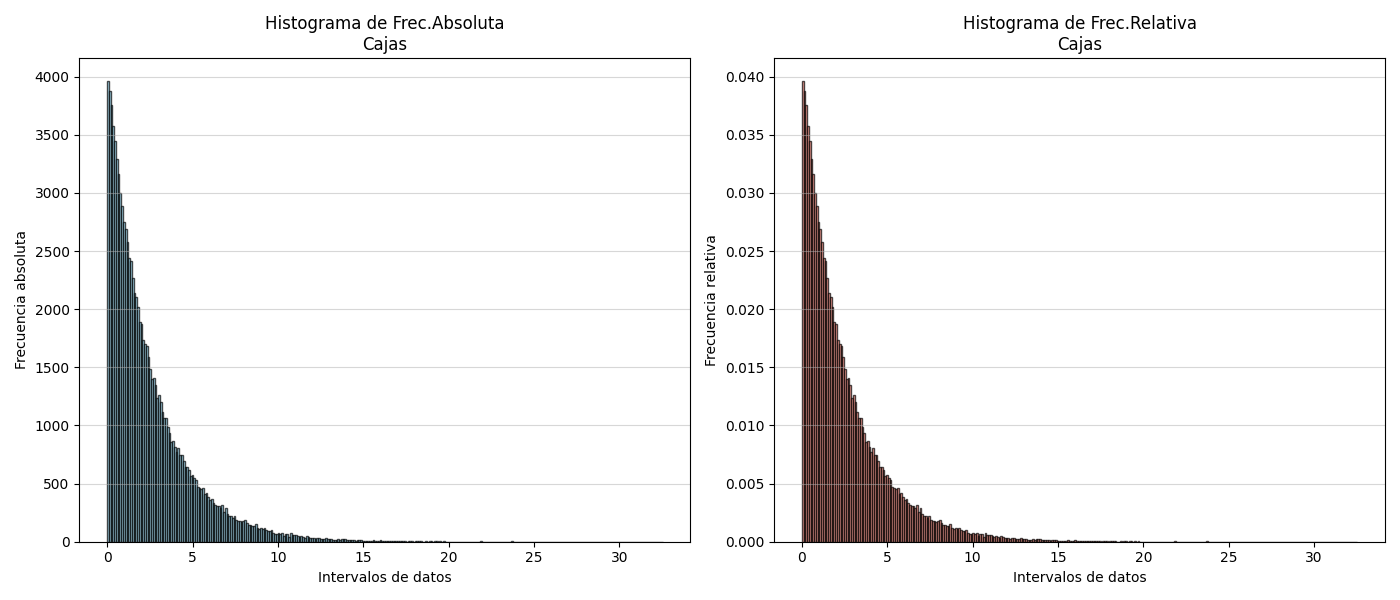
\includegraphics[width=\linewidth]{Imágenes/frec/cajaFrec.png}
        \caption{Histograma de frecuencias}
        \label{fig:frec_cajas}
    \end{subfigure}
    \quad
    \begin{subfigure}{0.40\textwidth}
        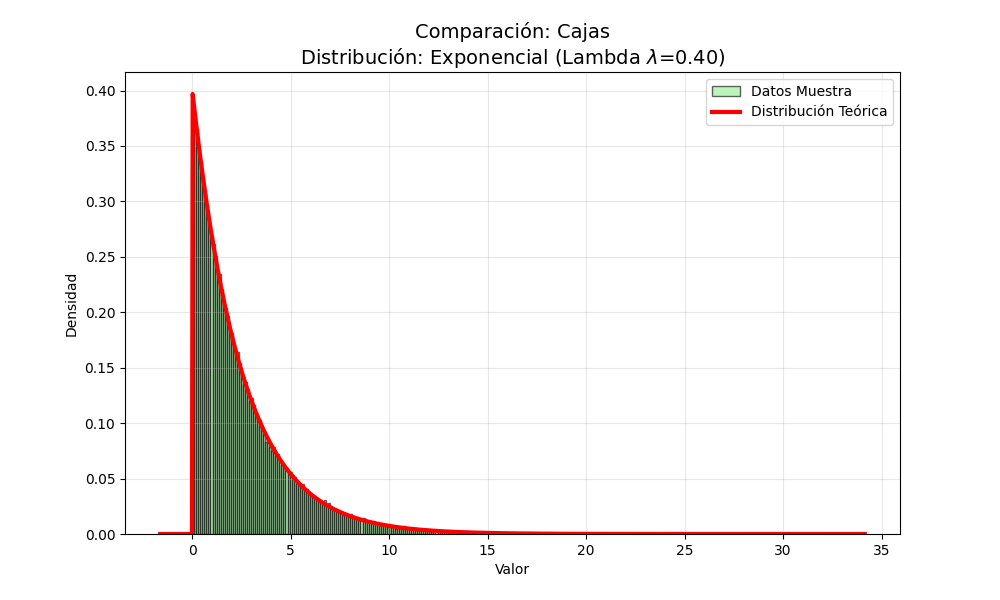
\includegraphics[width=\linewidth]{Imágenes/compara/cajaCompara.png}
        \caption{Comparación de la muestra}
        \label{fig:compara_cajas}
    \end{subfigure}
    \caption{Histogramas para el servicio de cajas.}
    \label{fig:hist_cajas}
\end{figure}

\begin{figure}[H]
    \centering
    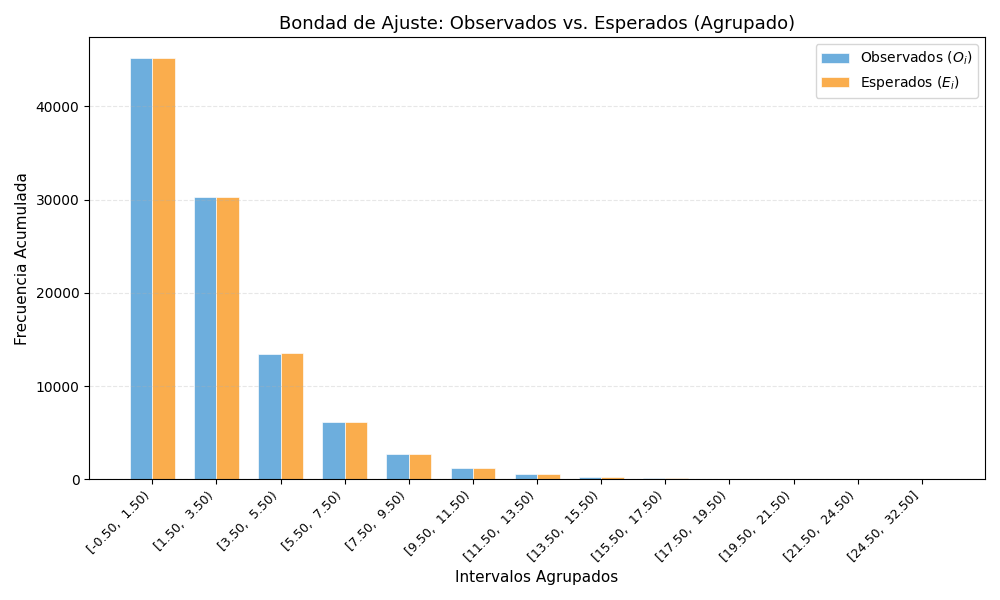
\includegraphics[width=0.5\textwidth]{Imágenes/obsEspe/cajasObsEspe.png}
    \caption{Observados vs Esperados para cajas.}
    \label{fig:obsEspe_cajas}
\end{figure}

\begin{center}
    \textbf{Datos de la muestra (Cajas):}
    \vspace{0.2cm}
    \\Media (\(\mu\)): 2.4984 \quad | \quad Lambda (\(\lambda\)): 0.40
\end{center}

\newpage
\subsubsection*{1.1.2.\hspace{0.5em} Planteamiento de hipótesis}
En base al análisis de los datos, se proponen las siguientes hipótesis:
\begin{center}
    \textbf{\(H_0\):} Esta es una distribución \textbf{Exponencial} con
    \(\lambda = 0.40\).\\[0.5em]
    \textbf{\(H_1\):} La anterior \textbf{NO} es una buena descripción
    de la distribución.
\end{center}

\vspace{0.3cm}
\noindent \textbf{Criterios de decisión:}
\begin{itemize}
    \item Para la prueba \(\chi^2\): un nivel de confianza de \(95\%\) (\(\alpha = 0.05\)).
    \item Para la prueba \textit{Kolmogorov-Smirnov}: un nivel de confianza de \(95\%\) (\(\alpha = 0.05\)).
    \item Si \(\chi^2 \leq \text{valorCritico}\) y \(d \leq \text{valorCritico}\), entonces se acepta \(H_0\).
    \item Si no se cumple lo anterior, se rechaza la hipótesis nula.
\end{itemize}
\vspace{0.3cm}

\subsubsection*{1.1.3.\hspace{0.5em} Pruebas de bondad de ajuste}
\vspace{0.2cm}
\begin{minipage}{0.40\textwidth}
    \textbf{Función de Densidad (PDF):}
    \[
        f(x) = \lambda e^{-\lambda x}, \quad x \ge 0
    \]
\end{minipage}
\begin{minipage}{0.45\textwidth}
    \textbf{Función de Distribución (CDF):}
    \[
        F(x) = 1 - e^{-\lambda x}, \quad x \ge 0
    \]
\end{minipage}
\vspace{0.3cm}

\noindent
\begin{minipage}[t]{0.48\textwidth}
    \textbf{1. Prueba de \(\chi^2\)}
    \vspace{0.3cm}
    \begin{itemize}[itemsep=0.4em]
        \item \textbf{Calculado \(\chi^2\):} 27.4483
        \item \textbf{Valor crítico:} 43.7730
    \end{itemize}

    \begin{center}
        \vspace{0.5cm}
        \(27.4483 \leq 43.7730\)
        \vspace{0.1cm}
        \\\textbf{Resultado: }
        \textcolor{green!60!black}{\textbf{Aprobado}}
    \end{center}

    \vspace{0.8cm}

    \textbf{2. Prueba de Kolmogorov--Smirnov}
    \vspace{0.3cm}
    \begin{itemize}[itemsep=0.4em]
        \item \textbf{Calculado \(D\):} 0.001403
        \item \textbf{Valor crítico:} 0.004301
    \end{itemize}
    \begin{center}
        \vspace{0.5cm}
        \(0.0014 \leq 0.0043\)
        \vspace{0.1cm}
        \\\textbf{Resultado: }
        \textcolor{green!60!black}{\textbf{Aprobado}}
    \end{center}

\end{minipage}
\hfill
\begin{minipage}[t]{0.48\textwidth}
    \vspace{0pt}
    \centering
    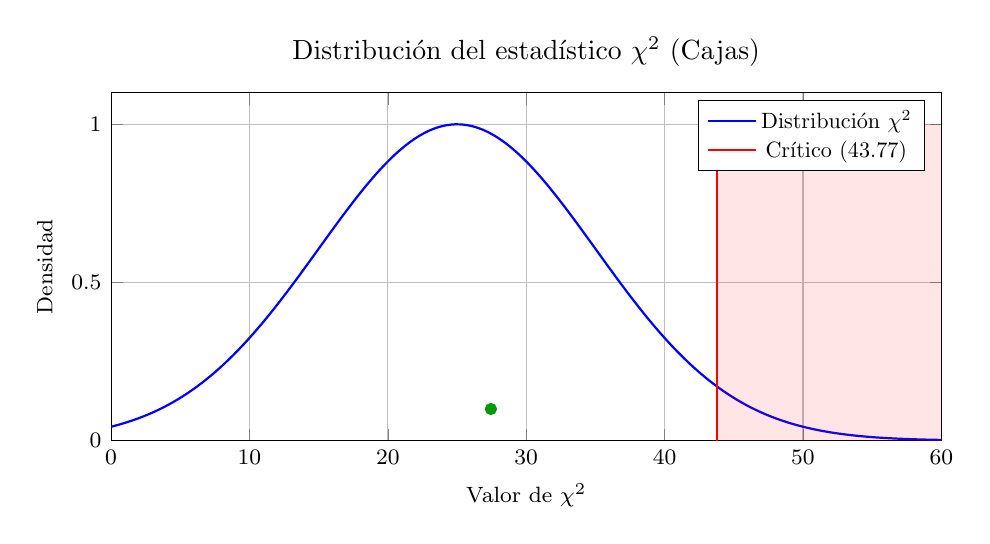
\begin{tikzpicture}
        \begin{axis}[
                width=\textwidth,
                height=6cm,
                title={Distribución del estadístico \(\chi^2\) (Cajas)},
                xlabel={Valor de \(\chi^2\)},
                ylabel={Densidad},
                xmin=0, xmax=60,
                ymin=0, ymax=1.1,
                grid=both,
                domain=0:60,
                samples=100,
                label style={font=\footnotesize},
                tick label style={font=\footnotesize},
                legend style={
                        nodes={scale=0.8, transform shape},
                        at={(0.98,0.98)},
                        anchor=north east
                    },]
            \addplot[blue, thick, smooth]
            {exp(-0.5*((x-25)/10)^2)};
            \addlegendentry{Distribución \(\chi^2\)}
            \addplot[red, thick]
            coordinates {(43.7729, 0) (43.7729, 1)};
            \addlegendentry{Crítico (43.77)}
            \addplot[fill=red, opacity=0.1]
            coordinates {(43.7729, 0) (60, 0) (60, 1) (43.7729, 1)};
            \addplot[
                mark=*,
                only marks,
                mark options={color=green!60!black, fill=green!60!black}
            ] coordinates {(27.4483, 0.1)};
        \end{axis}
    \end{tikzpicture}
\end{minipage}
\vspace{0.5cm}

\begin{center}
    Dado que ambas pruebas fueron aprobadas,
    \textbf{se acepta \(H_0\)}.
\end{center}


% Refrescos
\subsection{Servidor refrescos}
\subsubsection*{1.2.1.\hspace{0.5em} Análisis de frecuencias}
\begin{figure}[H]
    \centering
    \begin{subfigure}{0.55\textwidth}
        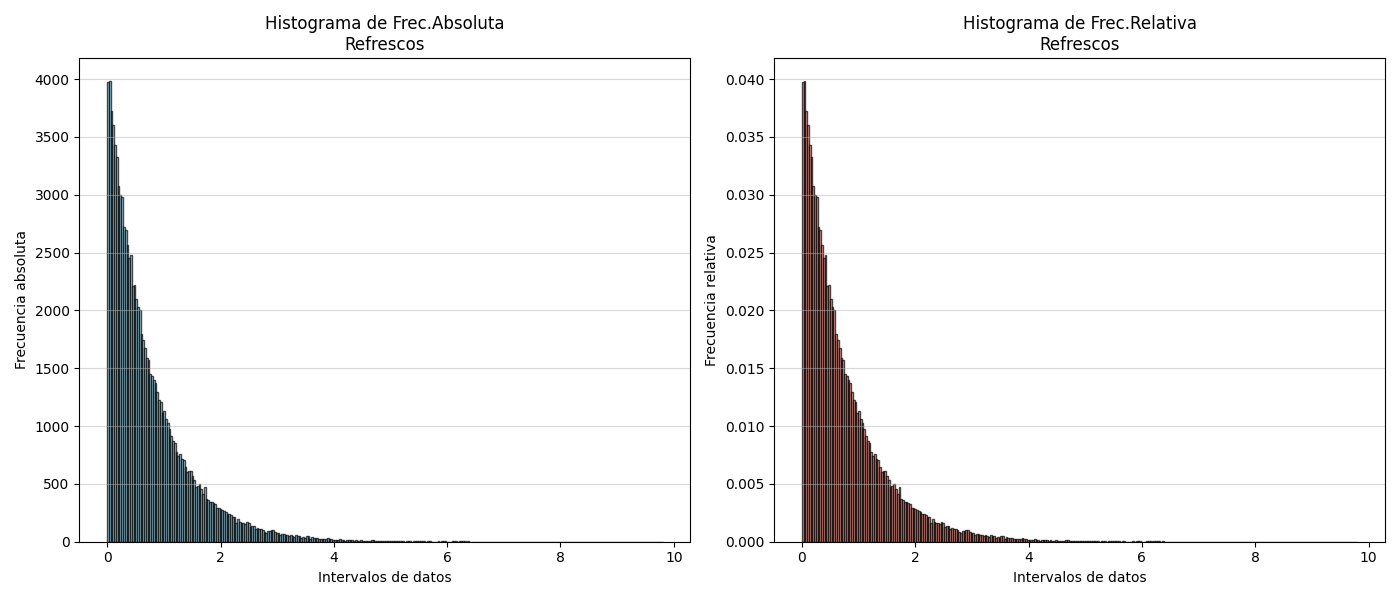
\includegraphics[width=\linewidth]{Imágenes/frec/refreFrec.png}
        \caption{Histograma de frecuencias}
        \label{fig:frec_refrescos}
    \end{subfigure}
    \quad
    \begin{subfigure}{0.40\textwidth}
        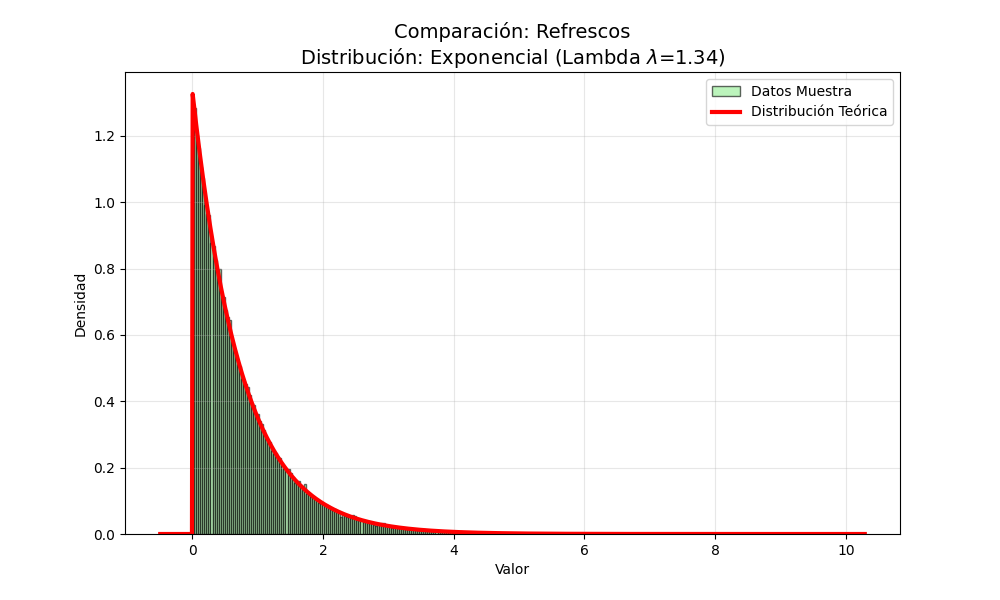
\includegraphics[width=\linewidth]{Imágenes/compara/refreCompara.png}
        \caption{Comparación de la muestra}
        \label{fig:compara_refrescos}
    \end{subfigure}
    \caption{Histogramas para el servicio de refrescos.}
    \label{fig:hist_refrescos}
\end{figure}

\begin{figure}[H]
    \centering
    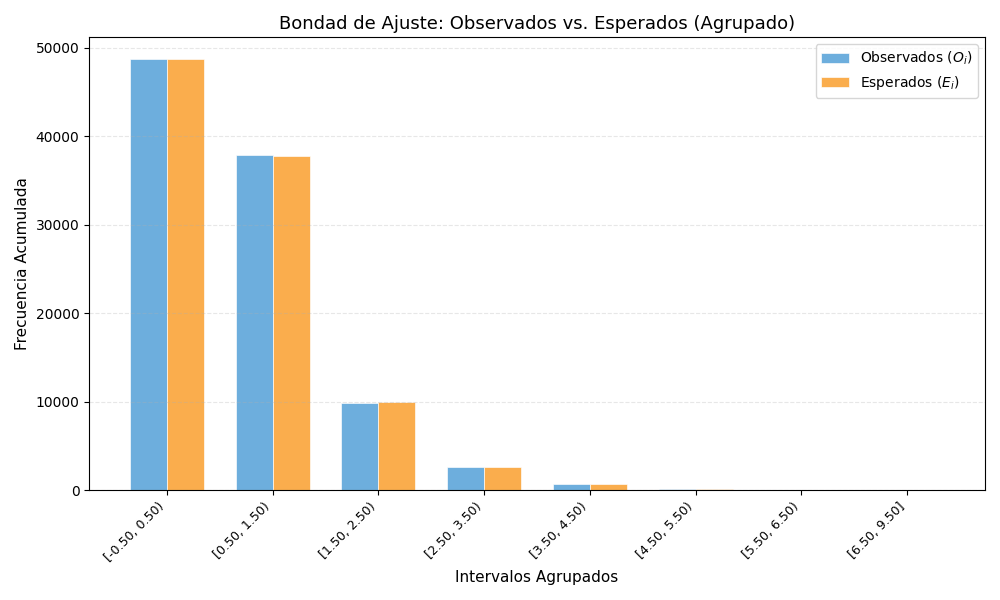
\includegraphics[width=0.5\textwidth]{Imágenes/obsEspe/refreObsEspe.png}
    \caption{Observados vs Esperados para refrescos.}
    \label{fig:obsEspe_refrescos}
\end{figure}

\begin{center}
    \textbf{Datos de la muestra (Refrescos):}
    \vspace{0.2cm}
    \\Media (\(\mu\)): 0.7477 \quad | \quad Lambda (\(\lambda\)): 1.34
\end{center}

\newpage
\subsubsection*{1.2.2.\hspace{0.5em} Planteamiento de hipótesis}
En base al análisis de los datos, se proponen las siguientes hipótesis:
\begin{center}
    \textbf{\(H_0\):} Esta es una distribución \textbf{Exponencial} con
    \(\lambda = 1.34\).\\[0.5em]
    \textbf{\(H_1\):} La anterior \textbf{NO} es una buena descripción
    de la distribución.
\end{center}

\vspace{0.3cm}
\noindent \textbf{Criterios de decisión:}
\begin{itemize}
    \item Para la prueba \(\chi^2\): un nivel de confianza de \(95\%\) (\(\alpha = 0.05\)).
    \item Para la prueba \textit{Kolmogorov-Smirnov}: un nivel de confianza de \(95\%\) (\(\alpha = 0.05\)).
    \item Si \(\chi^2 \leq \text{valorCritico}\) y \(d \leq \text{valorCritico}\), entonces se acepta \(H_0\).
    \item Si no se cumple lo anterior, se rechaza la hipótesis nula.
\end{itemize}
\vspace{0.3cm}

\subsubsection*{1.2.3.\hspace{0.5em} Pruebas de bondad de ajuste}
\vspace{0.2cm}
\begin{minipage}{0.40\textwidth}
    \textbf{Función de Densidad (PDF):}
    \[
        f(x) = \lambda e^{-\lambda x}, \quad x \ge 0
    \]
\end{minipage}
\begin{minipage}{0.45\textwidth}
    \textbf{Función de Distribución (CDF):}
    \[
        F(x) = 1 - e^{-\lambda x}, \quad x \ge 0
    \]
\end{minipage}
\vspace{0.3cm}

\noindent
\begin{minipage}[t]{0.48\textwidth}
    \textbf{1. Prueba de \(\chi^2\)}
    \vspace{0.3cm}
    \begin{itemize}[itemsep=0.4em]
        \item \textbf{Calculado \(\chi^2\):} 5.4405
        \item \textbf{Valor crítico:} 14.0671
    \end{itemize}

    \begin{center}
        \vspace{0.5cm}
        \(5.4405 \leq 14.0671\)
        \vspace{0.1cm}
        \\\textbf{Resultado: }
        \textcolor{green!60!black}{\textbf{Aprobado}}
    \end{center}

    \vspace{0.8cm}

    \textbf{2. Prueba de Kolmogorov--Smirnov}
    \vspace{0.3cm}
    \begin{itemize}[itemsep=0.4em]
        \item \textbf{Calculado \(D\):} 0.001934
        \item \textbf{Valor crítico:} 0.004301
    \end{itemize}
    \begin{center}
        \vspace{0.5cm}
        \(0.0019 \leq 0.0043\)
        \vspace{0.1cm}
        \\\textbf{Resultado: }
        \textcolor{green!60!black}{\textbf{Aprobado}}
    \end{center}

\end{minipage}
\hfill
\begin{minipage}[t]{0.48\textwidth}
    \vspace{0pt}
    \centering
    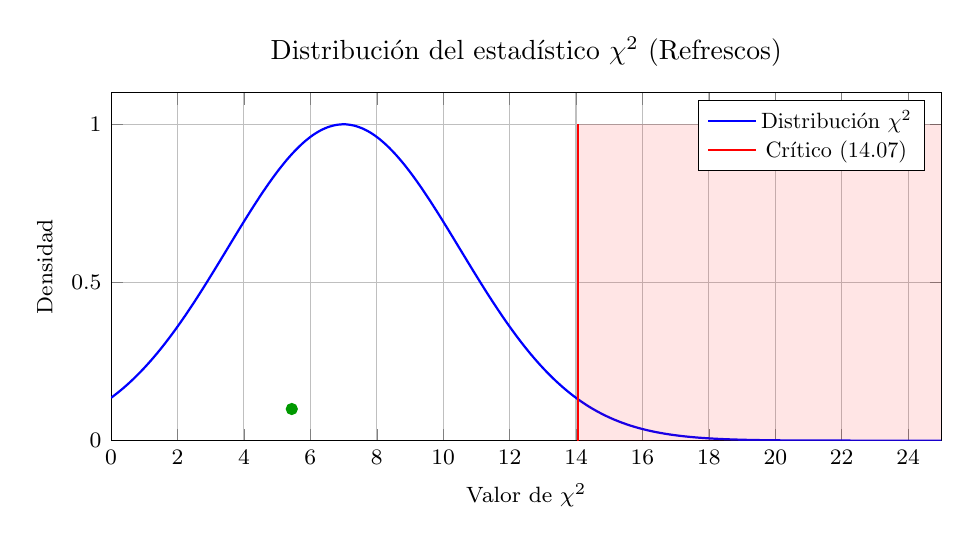
\begin{tikzpicture}
        \begin{axis}[
                width=\textwidth,
                height=6cm,
                title={Distribución del estadístico \(\chi^2\) (Refrescos)},
                xlabel={Valor de \(\chi^2\)},
                ylabel={Densidad},
                xmin=0, xmax=25,
                ymin=0, ymax=1.1,
                grid=both,
                domain=0:25,
                samples=100,
                label style={font=\footnotesize},
                tick label style={font=\footnotesize},
                legend style={
                        nodes={scale=0.8, transform shape},
                        at={(0.98,0.98)},
                        anchor=north east
                    },]
            \addplot[blue, thick, smooth]
            {exp(-0.5*((x-7)/3.5)^2)};
            \addlegendentry{Distribución \(\chi^2\)}
            \addplot[red, thick]
            coordinates {(14.0671, 0) (14.0671, 1)};
            \addlegendentry{Crítico (14.07)}
            \addplot[fill=red, opacity=0.1]
            coordinates {(14.0671, 0) (25, 0) (25, 1) (14.0671, 1)};
            \addplot[
                mark=*,
                only marks,
                mark options={color=green!60!black, fill=green!60!black}
            ] coordinates {(5.4405, 0.1)};
        \end{axis}
    \end{tikzpicture}
\end{minipage}
\vspace{0.5cm}

\begin{center}
    Dado que ambas pruebas fueron aprobadas,
    \textbf{se acepta \(H_0\)}.
\end{center}


% Llegadas
\subsection{Servidor llegadas}
\subsubsection*{1.3.1.\hspace{0.5em} Análisis de frecuencias}
\begin{figure}[H]
    \centering
    \begin{subfigure}{0.55\textwidth}
        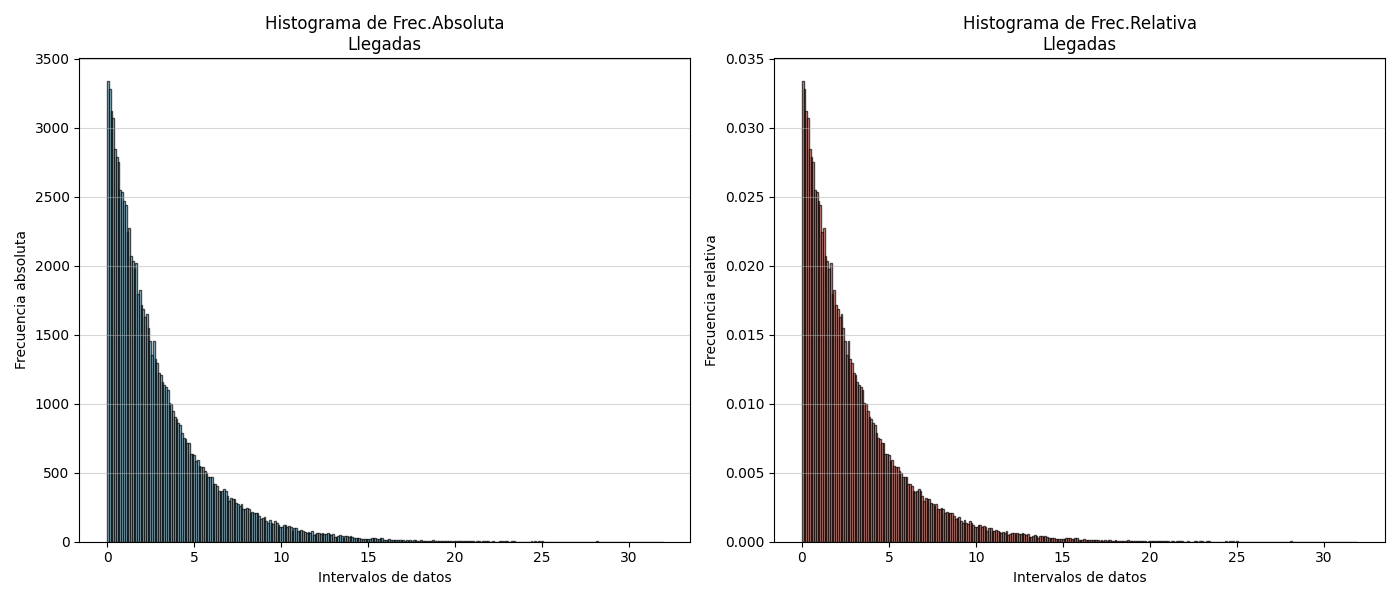
\includegraphics[width=\linewidth]{Imágenes/frec/llegadaFrec.png}
        \caption{Histograma de frecuencias}
        \label{fig:frec_llegadas}
    \end{subfigure}
    \quad
    \begin{subfigure}{0.40\textwidth}
        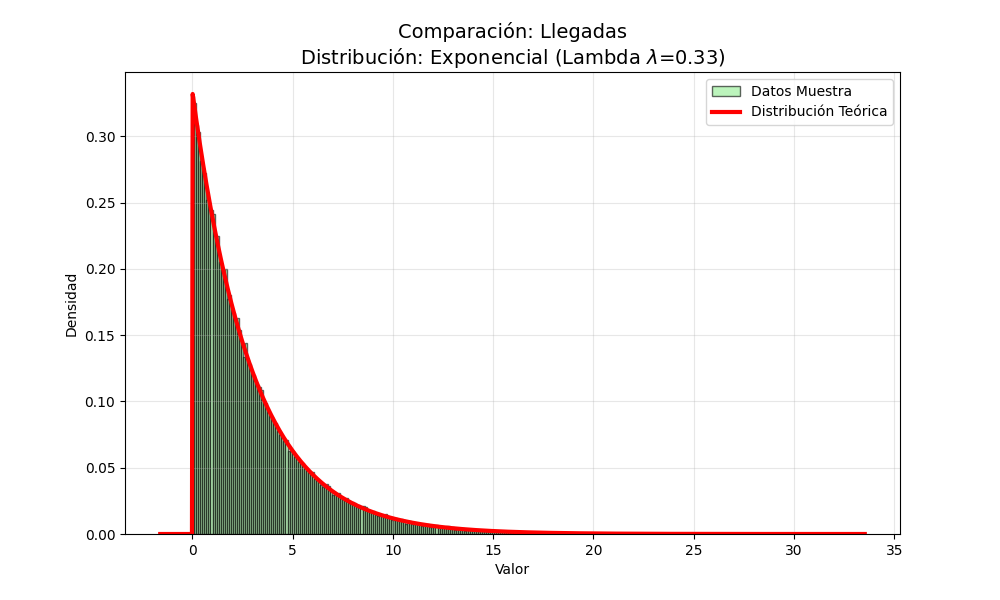
\includegraphics[width=\linewidth]{Imágenes/compara/llegadaCompara.png}
        \caption{Comparación de la muestra}
        \label{fig:compara_llegadas}
    \end{subfigure}
    \caption{Histogramas para el servicio de llegadas.}
    \label{fig:hist_llegadas}
\end{figure}

\begin{figure}[H]
    \centering
    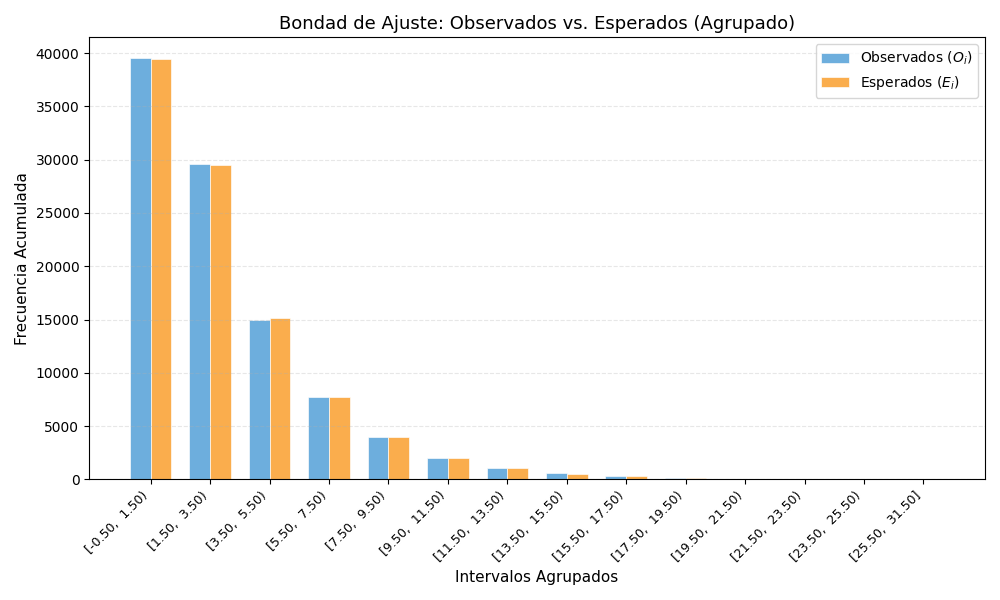
\includegraphics[width=0.5\textwidth]{Imágenes/obsEspe/llegadaObsEspe.png}
    \caption{Observados vs Esperados para llegadas.}
    \label{fig:obsEspe_llegadas}
\end{figure}

\begin{center}
    \textbf{Datos de la muestra (Llegadas):}
    \vspace{0.2cm}
    \\Media (\(\mu\)): 2.9913 \quad | \quad Lambda (\(\lambda\)): 0.33
\end{center}

\newpage
\subsubsection*{1.3.2.\hspace{0.5em} Planteamiento de hipótesis}
En base al análisis de los datos, se proponen las siguientes hipótesis:
\begin{center}
    \textbf{\(H_0\):} Esta es una distribución \textbf{Exponencial} con
    \(\lambda = 0.33\).\\[0.5em]
    \textbf{\(H_1\):} La anterior \textbf{NO} es una buena descripción
    de la distribución.
\end{center}

\vspace{0.3cm}
\noindent \textbf{Criterios de decisión:}
\begin{itemize}
    \item Para la prueba \(\chi^2\): un nivel de confianza de \(95\%\) (\(\alpha = 0.05\)).
    \item Para la prueba \textit{Kolmogorov-Smirnov}: un nivel de confianza de \(95\%\) (\(\alpha = 0.05\)).
    \item Si \(\chi^2 \leq \text{valorCritico}\) y \(d \leq \text{valorCritico}\), entonces se acepta \(H_0\).
    \item Si no se cumple lo anterior, se rechaza la hipótesis nula.
\end{itemize}
\vspace{0.3cm}

\subsubsection*{1.3.3.\hspace{0.5em} Pruebas de bondad de ajuste}
\vspace{0.2cm}
\begin{minipage}{0.40\textwidth}
    \textbf{Función de Densidad (PDF):}
    \[
        f(x) = \lambda e^{-\lambda x}, \quad x \ge 0
    \]
\end{minipage}
\begin{minipage}{0.45\textwidth}
    \textbf{Función de Distribución (CDF):}
    \[
        F(x) = 1 - e^{-\lambda x}, \quad x \ge 0
    \]
\end{minipage}
\vspace{0.3cm}

\noindent
\begin{minipage}[t]{0.48\textwidth}
    \textbf{1. Prueba de \(\chi^2\)}
    \vspace{0.3cm}
    \begin{itemize}[itemsep=0.4em]
        \item \textbf{Calculado \(\chi^2\):} 21.3846
        \item \textbf{Valor crítico:} 42.5569
    \end{itemize}

    \begin{center}
        \vspace{0.5cm}
        \(21.3846 \leq 42.5569\)
        \vspace{0.1cm}
        \\\textbf{Resultado: }
        \textcolor{green!60!black}{\textbf{Aprobado}}
    \end{center}

    \vspace{0.8cm}

    \textbf{2. Prueba de Kolmogorov--Smirnov}
    \vspace{0.3cm}
    \begin{itemize}[itemsep=0.4em]
        \item \textbf{Calculado \(D\):} 0.001950
        \item \textbf{Valor crítico:} 0.004301
    \end{itemize}
    \begin{center}
        \vspace{0.5cm}
        \(0.0019 \leq 0.0043\)
        \vspace{0.1cm}
        \\\textbf{Resultado: }
        \textcolor{green!60!black}{\textbf{Aprobado}}
    \end{center}

\end{minipage}
\hfill
\begin{minipage}[t]{0.48\textwidth}
    \vspace{0pt}
    \centering
    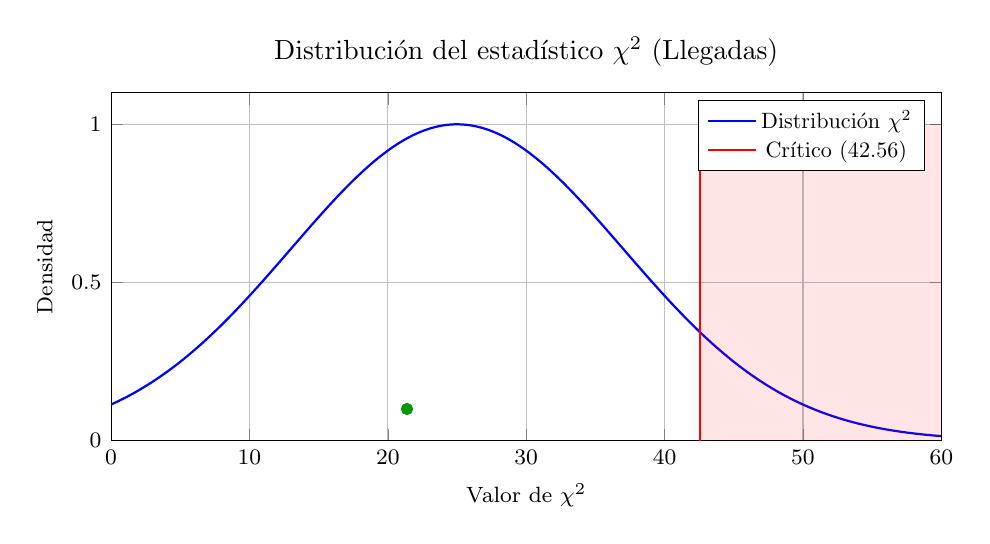
\begin{tikzpicture}
        \begin{axis}[
                width=\textwidth,
                height=6cm,
                title={Distribución del estadístico \(\chi^2\) (Llegadas)},
                xlabel={Valor de \(\chi^2\)},
                ylabel={Densidad},
                xmin=0, xmax=60,
                ymin=0, ymax=1.1,
                grid=both,
                domain=0:60,
                samples=100,
                label style={font=\footnotesize},
                tick label style={font=\footnotesize},
                legend style={
                        nodes={scale=0.8, transform shape},
                        at={(0.98,0.98)},
                        anchor=north east
                    },]
            \addplot[blue, thick, smooth]
            {exp(-0.5*((x-25)/12)^2)};
            \addlegendentry{Distribución \(\chi^2\)}
            \addplot[red, thick]
            coordinates {(42.5569, 0) (42.5569, 1)};
            \addlegendentry{Crítico (42.56)}
            \addplot[fill=red, opacity=0.1]
            coordinates {(42.5569, 0) (60, 0) (60, 1) (42.5569, 1)};
            \addplot[
                mark=*,
                only marks,
                mark options={color=green!60!black, fill=green!60!black}
            ] coordinates {(21.3846, 0.1)};
        \end{axis}
    \end{tikzpicture}
\end{minipage}
\vspace{0.5cm}

\begin{center}
    Dado que ambas pruebas fueron aprobadas,
    \textbf{se acepta \(H_0\)}.
\end{center}


% Postres
\subsection{Servidor postres}
\subsubsection*{1.4.1.\hspace{0.5em} Análisis de frecuencias}
\begin{figure}[H]
    \centering
    \begin{subfigure}{0.55\textwidth}
        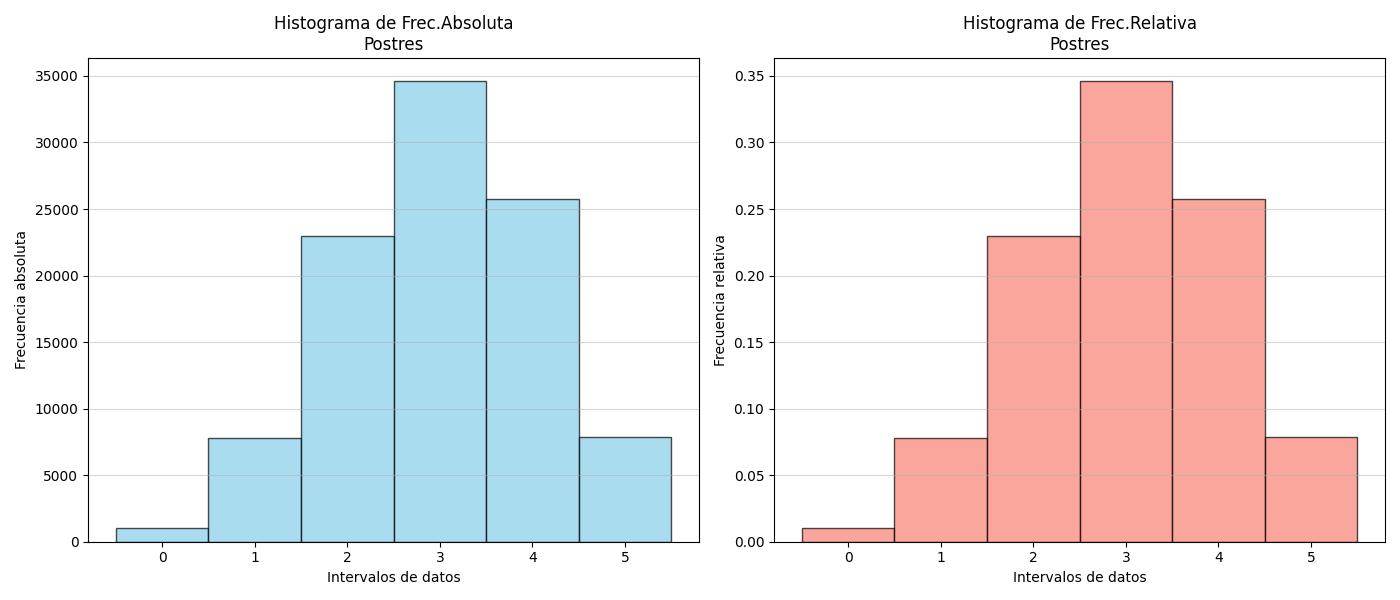
\includegraphics[width=\linewidth]{Imágenes/frec/postreFrec.png}
        \caption{Histograma de frecuencias}
        \label{fig:frec_postres}
    \end{subfigure}
    \quad
    \begin{subfigure}{0.40\textwidth}
        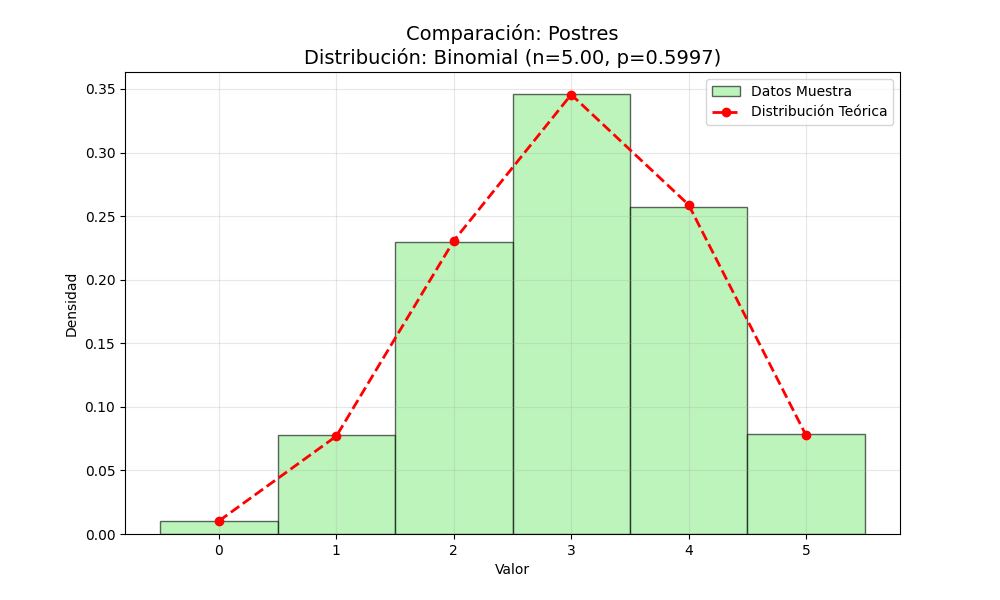
\includegraphics[width=\linewidth]{Imágenes/compara/postreCompara.png}
        \caption{Comparación de la muestra}
        \label{fig:compara_postres}
    \end{subfigure}
    \caption{Histogramas para el servicio de postres.}
    \label{fig:hist_postres}
\end{figure}

\begin{figure}[H]
    \centering
    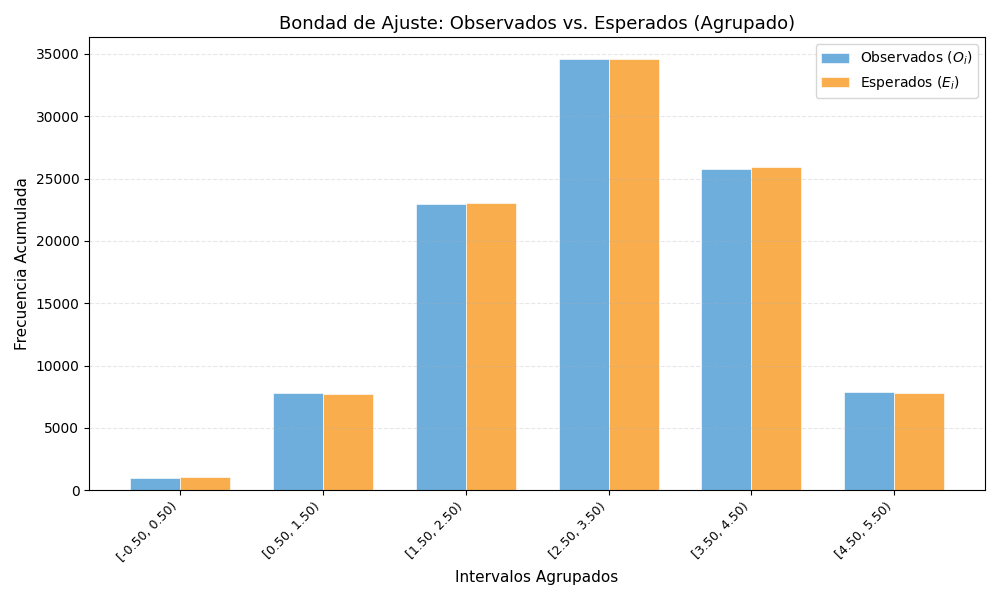
\includegraphics[width=0.5\textwidth]{Imágenes/obsEspe/postresObsEspe.png}
    \caption{Observados vs Esperados para postres.}
    \label{fig:obsEspe_postres}
\end{figure}

\begin{center}
    \textbf{Datos de la muestra (Postres):}
    \vspace{0.2cm}
    \\Parámetro (\textit{n}): 5 \quad | \quad Probabilidad (\textit{p}): 0.5997
\end{center}

\newpage
\subsubsection*{1.4.2.\hspace{0.5em} Planteamiento de hipótesis}
En base al análisis de los datos, se proponen las siguientes hipótesis:
\begin{center}
    \textbf{\(H_0\):} Esta es una distribución \textbf{Binomial} con
    \(n = 5\) y \(p = 0.5997\).\\[0.5em]
    \textbf{\(H_1\):} La anterior \textbf{NO} es una buena descripción
    de la distribución.
\end{center}

\noindent \textbf{Criterios de decisión:}
\begin{itemize}
    \item Para la prueba \(\chi^2\): un nivel de confianza de \(95\%\) (\(\alpha = 0.05\)).
    \item Para la prueba \textit{Kolmogorov-Smirnov}: un nivel de confianza de \(95\%\) (\(\alpha = 0.05\)).
    \item Si \(\chi^2 \leq \text{valorCritico}\) y \(d \leq \text{valorCritico}\), entonces se acepta \(H_0\).
    \item Si no se cumple lo anterior, se rechaza la hipótesis nula.
\end{itemize}

\subsubsection*{1.4.3.\hspace{0.5em} Pruebas de bondad de ajuste}
\vspace{0.2cm}
\begin{minipage}{0.40\textwidth}
    \textbf{Función de Masa (PMF):}
    \[
        P(X=k) = \binom{n}{k} p^k (1-p)^{n-k}
    \]
\end{minipage}
\begin{minipage}{0.45\textwidth}
    \textbf{Función de Distribución (CDF):}
    \[
        F(k) = \sum_{i=0}^{\lfloor k \rfloor} \binom{n}{i} p^i (1-p)^{n-i}
    \]
\end{minipage}

\noindent
\begin{minipage}[t]{0.48\textwidth}
    \textbf{1. Prueba de \(\chi^2\)}
    \vspace{0.3cm}
    \begin{itemize}[itemsep=0.4em]
        \item \textbf{Calculado \(\chi^2\):} 4.0657
        \item \textbf{Valor crítico:} 7.8147
    \end{itemize}

    \begin{center}
        \vspace{0.5cm}
        \(4.0657 \leq 7.8147\)
        \vspace{0.1cm}
        \\\textbf{Resultado: }
        \textcolor{green!60!black}{\textbf{Aprobado}}
    \end{center}

    \vspace{0.8cm}

    \textbf{2. Prueba de Kolmogorov--Smirnov}
    \vspace{0.3cm}
    \begin{itemize}[itemsep=0.4em]
        \item \textbf{Calculado \(D\):} 0.001106
        \item \textbf{Valor crítico:} 0.004301
    \end{itemize}
    \begin{center}
        \vspace{0.5cm}
        \(0.0011 \leq 0.0043\)
        \vspace{0.1cm}
        \\\textbf{Resultado: }
        \textcolor{green!60!black}{\textbf{Aprobado}}
    \end{center}

\end{minipage}
\hfill
\begin{minipage}[t]{0.48\textwidth}
    \vspace{0pt}
    \centering
    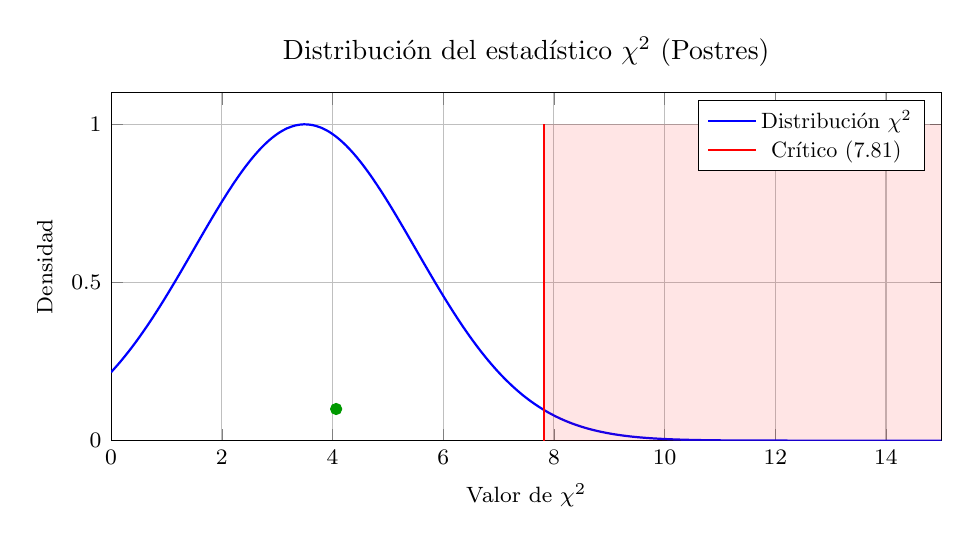
\begin{tikzpicture}
        \begin{axis}[
                width=\textwidth,
                height=6cm,
                title={Distribución del estadístico \(\chi^2\) (Postres)},
                xlabel={Valor de \(\chi^2\)},
                ylabel={Densidad},
                xmin=0, xmax=15,
                ymin=0, ymax=1.1,
                grid=both,
                domain=0:15,
                samples=100,
                label style={font=\footnotesize},
                tick label style={font=\footnotesize},
                legend style={
                        nodes={scale=0.8, transform shape},
                        at={(0.98,0.98)},
                        anchor=north east
                    },]
            \addplot[blue, thick, smooth]
            {exp(-0.5*((x-3.5)/2)^2)};
            \addlegendentry{Distribución \(\chi^2\)}
            \addplot[red, thick]
            coordinates {(7.8147, 0) (7.8147, 1)};
            \addlegendentry{Crítico (7.81)}
            \addplot[fill=red, opacity=0.1]
            coordinates {(7.8147, 0) (15, 0) (15, 1) (7.8147, 1)};
            \addplot[
                mark=*,
                only marks,
                mark options={color=green!60!black, fill=green!60!black}
            ] coordinates {(4.0657, 0.1)};
        \end{axis}
    \end{tikzpicture}
\end{minipage}
\vspace{0.5cm}

\begin{center}
    Dado que ambas pruebas fueron aprobadas,
    \textbf{se acepta \(H_0\)}.
\end{center}


% Ordenes
\subsection{Servidor ordenes}
\subsubsection*{1.5.1.\hspace{0.5em} Análisis de frecuencias}
\begin{figure}[H]
    \centering
    \begin{subfigure}{0.55\textwidth}
        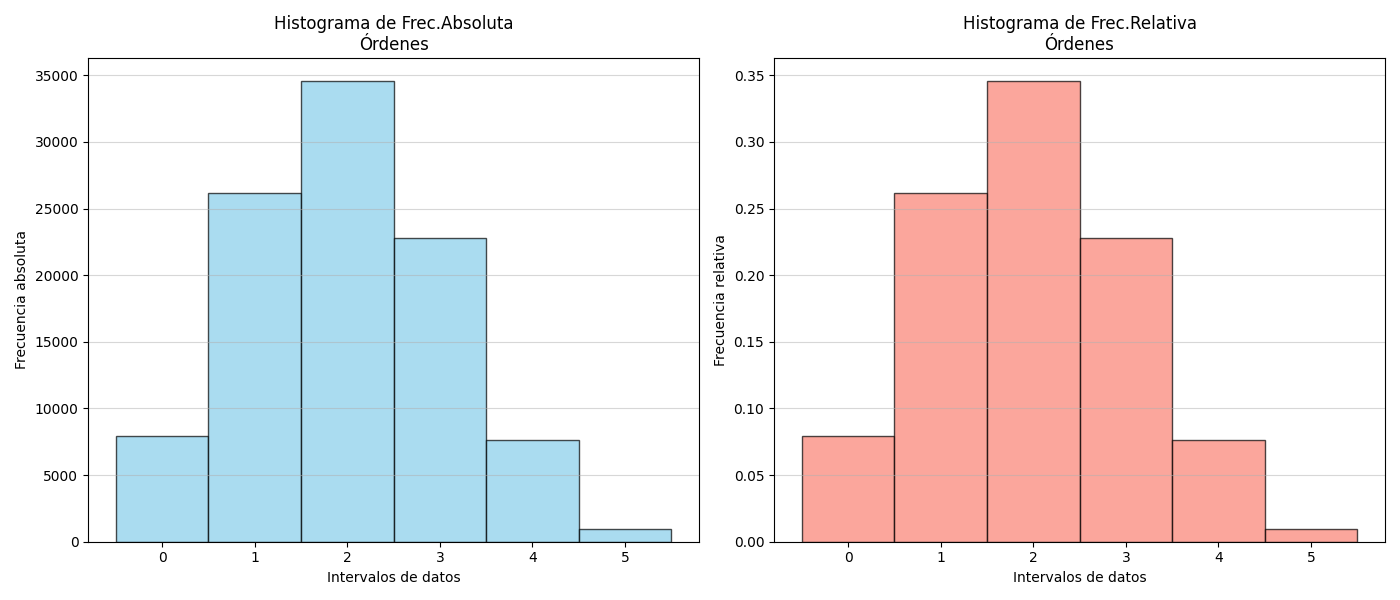
\includegraphics[width=\linewidth]{Imágenes/frec/ordenFrec.png}
        \caption{Histograma de frecuencias}
        \label{fig:frec_ordenes}
    \end{subfigure}
    \quad
    \begin{subfigure}{0.40\textwidth}
        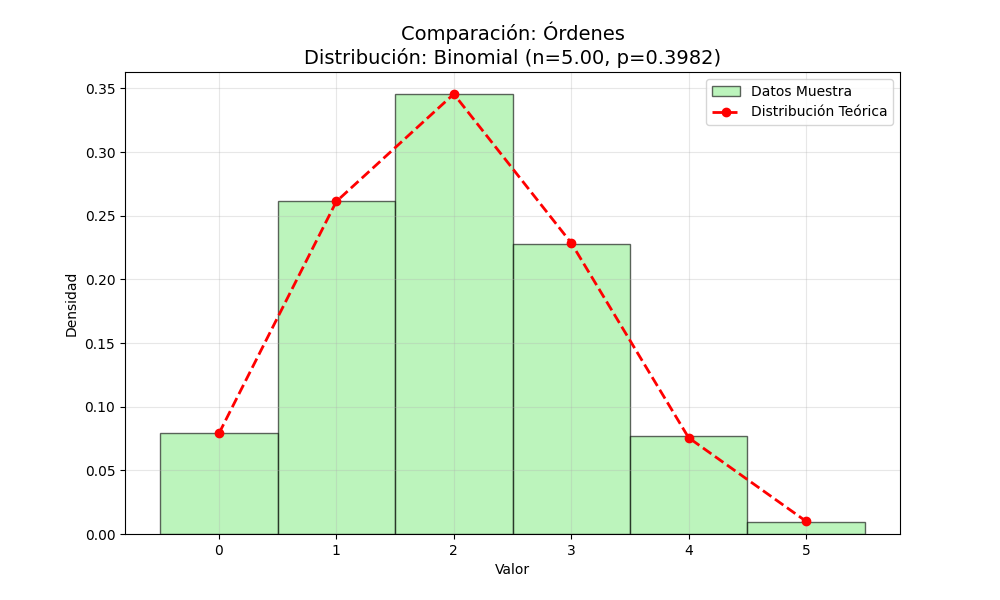
\includegraphics[width=\linewidth]{Imágenes/compara/ordenCompara.png}
        \caption{Comparación de la muestra}
        \label{fig:compara_ordenes}
    \end{subfigure}
    \caption{Histogramas para el servicio de ordenes.}
    \label{fig:hist_ordenes}
\end{figure}

\begin{figure}[H]
    \centering
    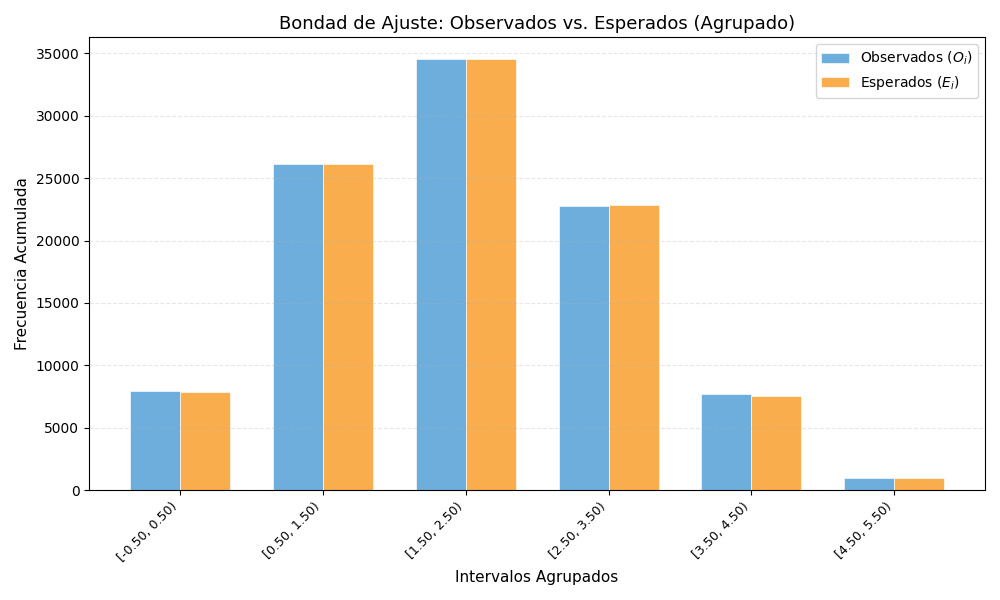
\includegraphics[width=0.5\textwidth]{Imágenes/obsEspe/ordenObsEspe.png}
    \caption{Observados vs Esperados para ordenes.}
    \label{fig:obsEspe_ordenes}
\end{figure}

\begin{center}
    \textbf{Datos de la muestra (Ordenes):}
    \vspace{0.2cm}
    \\Parámetro (\textit{n}): 5 \quad | \quad Probabilidad (\textit{p}): 0.3982
\end{center}

\newpage
\subsubsection*{1.5.2.\hspace{0.5em} Planteamiento de hipótesis}
En base al análisis de los datos, se proponen las siguientes hipótesis:
\begin{center}
    \textbf{\(H_0\):} Esta es una distribución \textbf{Binomial} con
    \(n = 5\) y \(p = 0.3982\).\\[0.5em]
    \textbf{\(H_1\):} La anterior \textbf{NO} es una buena descripción
    de la distribución.
\end{center}

\noindent \textbf{Criterios de decisión:}
\begin{itemize}
    \item Para la prueba \(\chi^2\): un nivel de confianza de \(95\%\) (\(\alpha = 0.05\)).
    \item Para la prueba \textit{Kolmogorov-Smirnov}: un nivel de confianza de \(95\%\) (\(\alpha = 0.05\)).
    \item Si \(\chi^2 \leq \text{valorCritico}\) y \(d \leq \text{valorCritico}\), entonces se acepta \(H_0\).
    \item Si no se cumple lo anterior, se rechaza la hipótesis nula.
\end{itemize}

\subsubsection*{1.5.3.\hspace{0.5em} Pruebas de bondad de ajuste}
\vspace{0.2cm}
\begin{minipage}{0.40\textwidth}
    \textbf{Función de Masa (PMF):}
    \[
        P(X=k) = \binom{n}{k} p^k (1-p)^{n-k}
    \]
\end{minipage}
\begin{minipage}{0.45\textwidth}
    \textbf{Función de Distribución (CDF):}
    \[
        F(k) = \sum_{i=0}^{\lfloor k \rfloor} \binom{n}{i} p^i (1-p)^{n-i}
    \]
\end{minipage}

\noindent
\begin{minipage}[t]{0.48\textwidth}
    \textbf{1. Prueba de \(\chi^2\)}
    \vspace{0.3cm}
    \begin{itemize}[itemsep=0.4em]
        \item \textbf{Calculado \(\chi^2\):} 2.5103
        \item \textbf{Valor crítico:} 7.8147
    \end{itemize}

    \begin{center}
        \vspace{0.5cm}
        \(2.5103 \leq 7.8147\)
        \vspace{0.1cm}
        \\\textbf{Resultado: }
        \textcolor{green!60!black}{\textbf{Aprobado}}
    \end{center}

    \vspace{0.8cm}

    \textbf{2. Prueba de Kolmogorov--Smirnov}
    \vspace{0.3cm}
    \begin{itemize}[itemsep=0.4em]
        \item \textbf{Calculado \(D\):} 0.000812
        \item \textbf{Valor crítico:} 0.004301
    \end{itemize}
    \begin{center}
        \vspace{0.5cm}
        \(0.0008 \leq 0.0043\)
        \vspace{0.1cm}
        \\\textbf{Resultado: }
        \textcolor{green!60!black}{\textbf{Aprobado}}
    \end{center}

\end{minipage}
\hfill
\begin{minipage}[t]{0.48\textwidth}
    \vspace{0pt}
    \centering
    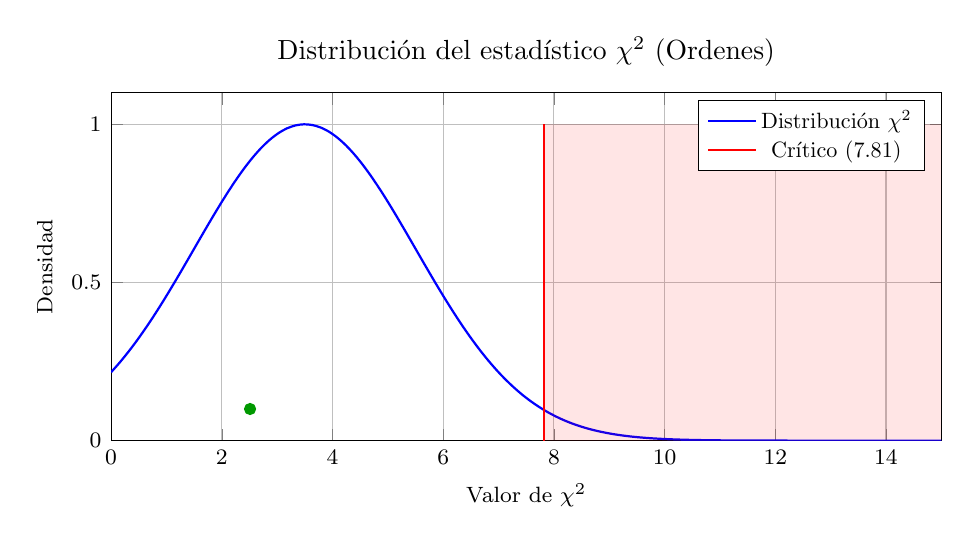
\begin{tikzpicture}
        \begin{axis}[
                width=\textwidth,
                height=6cm,
                title={Distribución del estadístico \(\chi^2\) (Ordenes)},
                xlabel={Valor de \(\chi^2\)},
                ylabel={Densidad},
                xmin=0, xmax=15,
                ymin=0, ymax=1.1,
                grid=both,
                domain=0:15,
                samples=100,
                label style={font=\footnotesize},
                tick label style={font=\footnotesize},
                legend style={
                        nodes={scale=0.8, transform shape},
                        at={(0.98,0.98)},
                        anchor=north east
                    },]
            \addplot[blue, thick, smooth]
            {exp(-0.5*((x-3.5)/2)^2)};
            \addlegendentry{Distribución \(\chi^2\)}
            \addplot[red, thick]
            coordinates {(7.8147, 0) (7.8147, 1)};
            \addlegendentry{Crítico (7.81)}
            \addplot[fill=red, opacity=0.1]
            coordinates {(7.8147, 0) (15, 0) (15, 1) (7.8147, 1)};
            \addplot[
                mark=*,
                only marks,
                mark options={color=green!60!black, fill=green!60!black}
            ] coordinates {(2.5103, 0.1)};
        \end{axis}
    \end{tikzpicture}
\end{minipage}
\vspace{0.5cm}

\begin{center}
    Dado que ambas pruebas fueron aprobadas,
    \textbf{se acepta \(H_0\)}.
\end{center}


% Pollo
\subsection{Servidor pollo}
\subsubsection*{1.6.1.\hspace{0.5em} Análisis de frecuencias}
\begin{figure}[H]
    \centering
    \begin{subfigure}{0.55\textwidth}
        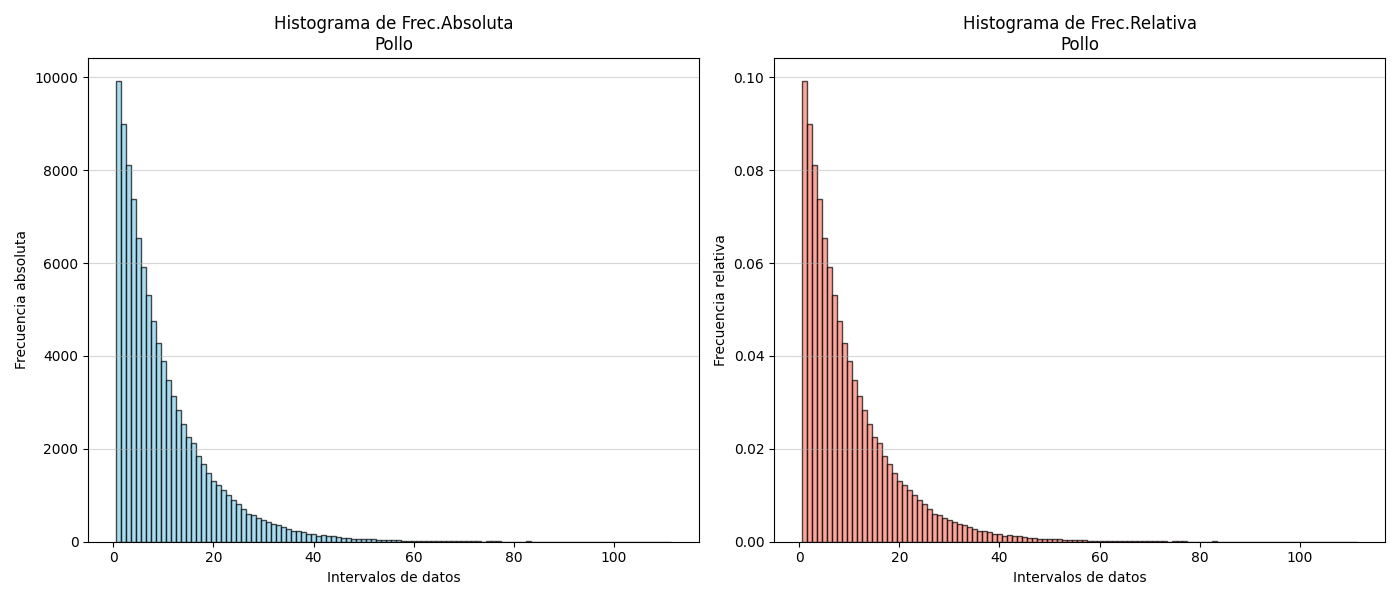
\includegraphics[width=\linewidth]{Imágenes/frec/polloFrec.png}
        \caption{Histograma de frecuencias}
        \label{fig:frec_pollo}
    \end{subfigure}
    \quad
    \begin{subfigure}{0.40\textwidth}
        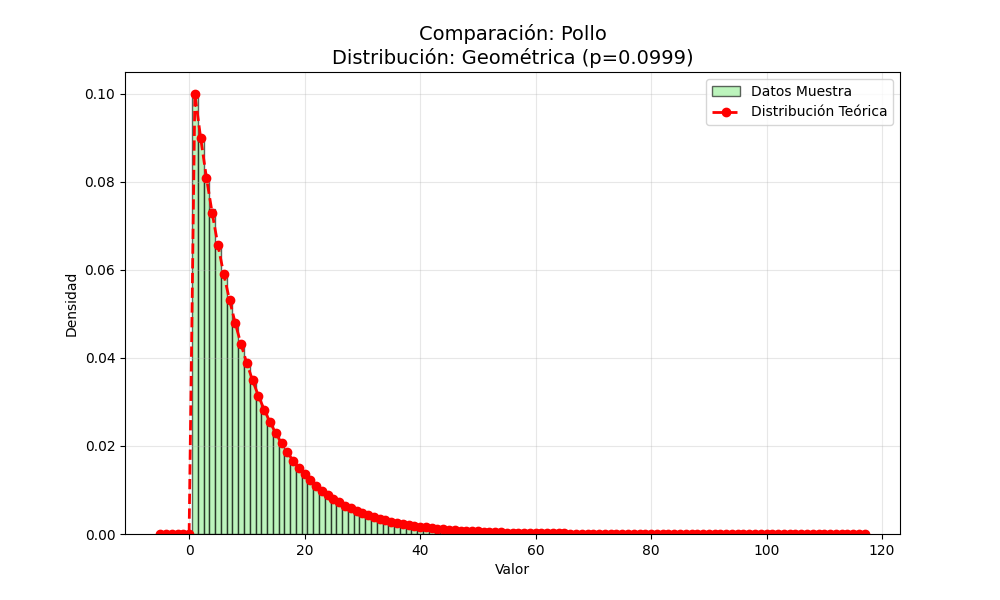
\includegraphics[width=\linewidth]{Imágenes/compara/polloCompara.png}
        \caption{Comparación de la muestra}
        \label{fig:compara_pollo}
    \end{subfigure}
    \caption{Histogramas para el servicio de pollo.}
    \label{fig:hist_pollo}
\end{figure}

\begin{figure}[H]
    \centering
    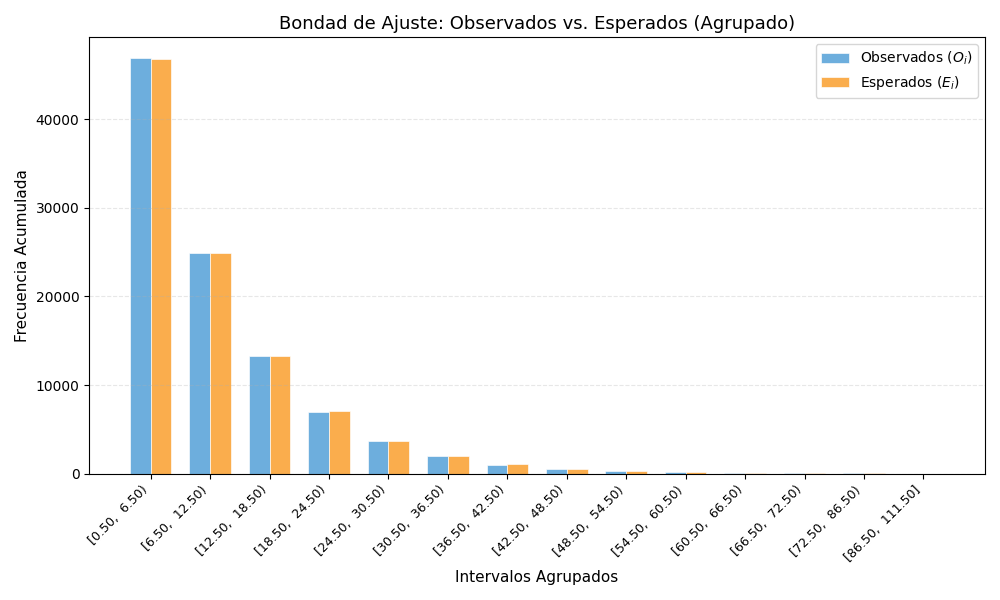
\includegraphics[width=0.5\textwidth]{Imágenes/obsEspe/polloObsEspe.png}
    \caption{Observados vs Esperados para pollo.}
    \label{fig:obsEspe_pollo}
\end{figure}

\begin{center}
    \textbf{Datos de la muestra (Pollo):}
    \vspace{0.2cm}
    \\Media (\(\mu\)): 10.0082 \quad | \quad Probabilidad (\textit{p}): 0.0999
\end{center}

\newpage
\subsubsection*{1.6.2.\hspace{0.5em} Planteamiento de hipótesis}
En base al análisis de los datos, se proponen las siguientes hipótesis:
\begin{center}
    \textbf{\(H_0\):} Esta es una distribución \textbf{Geométrica} con
    \(p = 0.0999\).\\[0.5em]
    \textbf{\(H_1\):} La anterior \textbf{NO} es una buena descripción
    de la distribución.
\end{center}

\vspace{0.3cm}
\noindent \textbf{Criterios de decisión:}
\begin{itemize}
    \item Para la prueba \(\chi^2\): un nivel de confianza de \(95\%\) (\(\alpha = 0.05\)).
    \item Para la prueba \textit{Kolmogorov-Smirnov}: un nivel de confianza de \(95\%\) (\(\alpha = 0.05\)).
    \item Si \(\chi^2 \leq \text{valorCritico}\) y \(d \leq \text{valorCritico}\), entonces se acepta \(H_0\).
    \item Si no se cumple lo anterior, se rechaza la hipótesis nula.
\end{itemize}
\vspace{0.3cm}

\subsubsection*{1.6.3.\hspace{0.5em} Pruebas de bondad de ajuste}
\vspace{0.2cm}
\begin{minipage}{0.40\textwidth}
    \textbf{Función de Masa (PMF):}
    \[
        P(X=k) = (1-p)^{k-1}p
    \]
\end{minipage}
\begin{minipage}{0.45\textwidth}
    \textbf{Función de Distribución (CDF):}
    \[
        F(k) = 1 - (1-p)^k
    \]
\end{minipage}
\vspace{0.3cm}

\noindent
\begin{minipage}[t]{0.48\textwidth}
    \textbf{1. Prueba de \(\chi^2\)}
    \vspace{0.3cm}
    \begin{itemize}[itemsep=0.4em]
        \item \textbf{Calculado \(\chi^2\):} 93.4691
        \item \textbf{Valor crítico:} 135.4802
    \end{itemize}

    \begin{center}
        \vspace{0.5cm}
        \(93.4691 \leq 135.4802\)
        \vspace{0.1cm}
        \\\textbf{Resultado: }
        \textcolor{green!60!black}{\textbf{Aprobado}}
    \end{center}

    \vspace{0.8cm}

    \textbf{2. Prueba de Kolmogorov--Smirnov}
    \vspace{0.3cm}
    \begin{itemize}[itemsep=0.4em]
        \item \textbf{Calculado \(D\):} 0.000823
        \item \textbf{Valor crítico:} 0.004301
    \end{itemize}
    \begin{center}
        \vspace{0.5cm}
        \(0.0008 \leq 0.0043\)
        \vspace{0.1cm}
        \\\textbf{Resultado: }
        \textcolor{green!60!black}{\textbf{Aprobado}}
    \end{center}

\end{minipage}
\hfill
\begin{minipage}[t]{0.48\textwidth}
    \vspace{0pt}
    \centering
    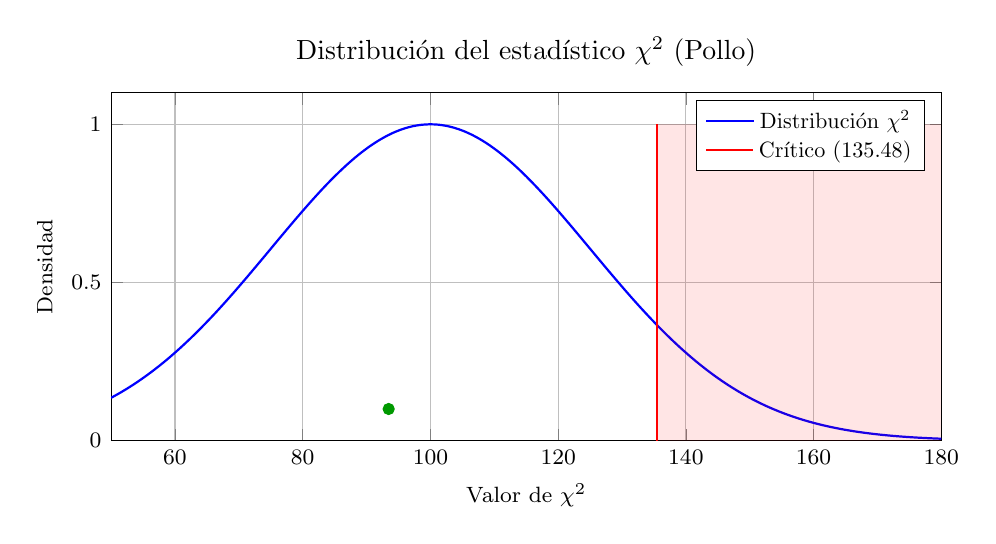
\begin{tikzpicture}
        \begin{axis}[
                width=\textwidth,
                height=6cm,
                title={Distribución del estadístico \(\chi^2\) (Pollo)},
                xlabel={Valor de \(\chi^2\)},
                ylabel={Densidad},
                xmin=50, xmax=180,
                ymin=0, ymax=1.1,
                grid=both,
                domain=50:180,
                samples=100,
                label style={font=\footnotesize},
                tick label style={font=\footnotesize},
                legend style={
                        nodes={scale=0.8, transform shape},
                        at={(0.98,0.98)},
                        anchor=north east
                    },]
            \addplot[blue, thick, smooth]
            {exp(-0.5*((x-100)/25)^2)};
            \addlegendentry{Distribución \(\chi^2\)}
            \addplot[red, thick]
            coordinates {(135.48, 0) (135.48, 1)};
            \addlegendentry{Crítico (135.48)}
            \addplot[fill=red, opacity=0.1]
            coordinates {(135.48, 0) (180, 0) (180, 1) (135.48, 1)};
            \addplot[
                mark=*,
                only marks,
                mark options={color=green!60!black, fill=green!60!black}
            ] coordinates {(93.46, 0.1)};
        \end{axis}
    \end{tikzpicture}
\end{minipage}
\vspace{0.5cm}

\begin{center}
    Dado que ambas pruebas fueron aprobadas,
    \textbf{se acepta \(H_0\)}.
\end{center}


% Freidora
\subsection{Servidor freidora}
\subsubsection*{1.7.1.\hspace{0.5em} Análisis de frecuencias}
\begin{figure}[H]
    \centering
    \begin{subfigure}{0.55\textwidth}
        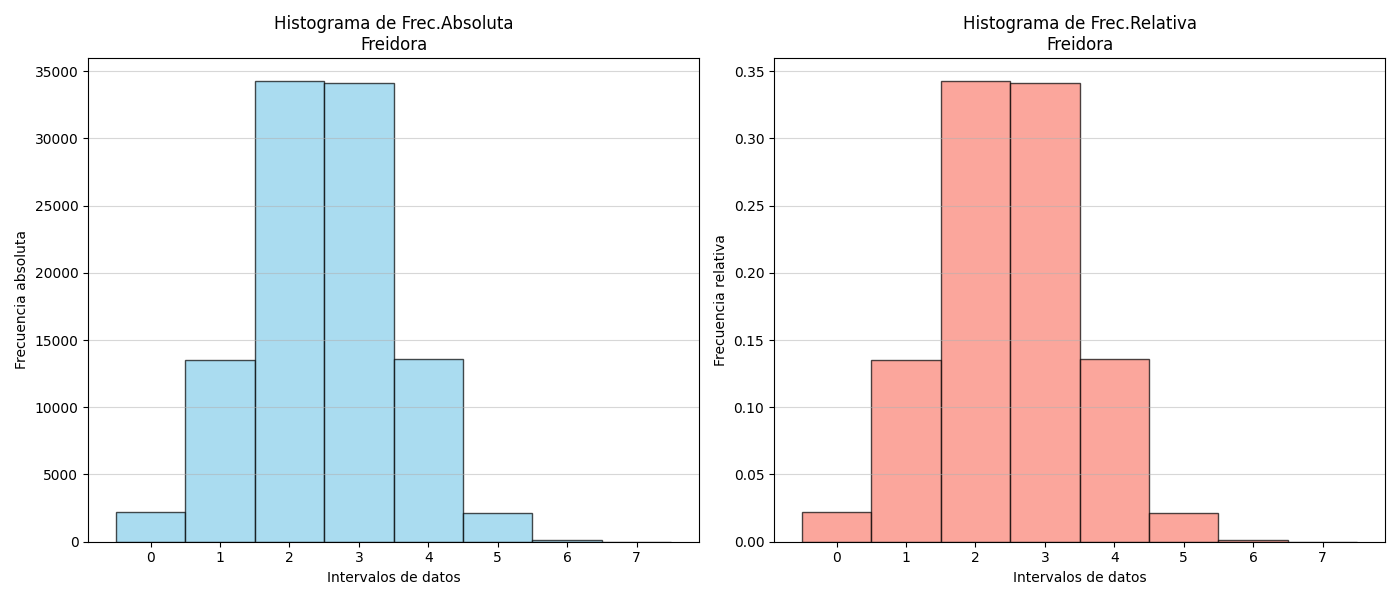
\includegraphics[width=\linewidth]{Imágenes/frec/freidoraFrec.png}
        \caption{Histograma de frecuencias}
        \label{fig:frec_freidora}
    \end{subfigure}
    \quad
    \begin{subfigure}{0.40\textwidth}
        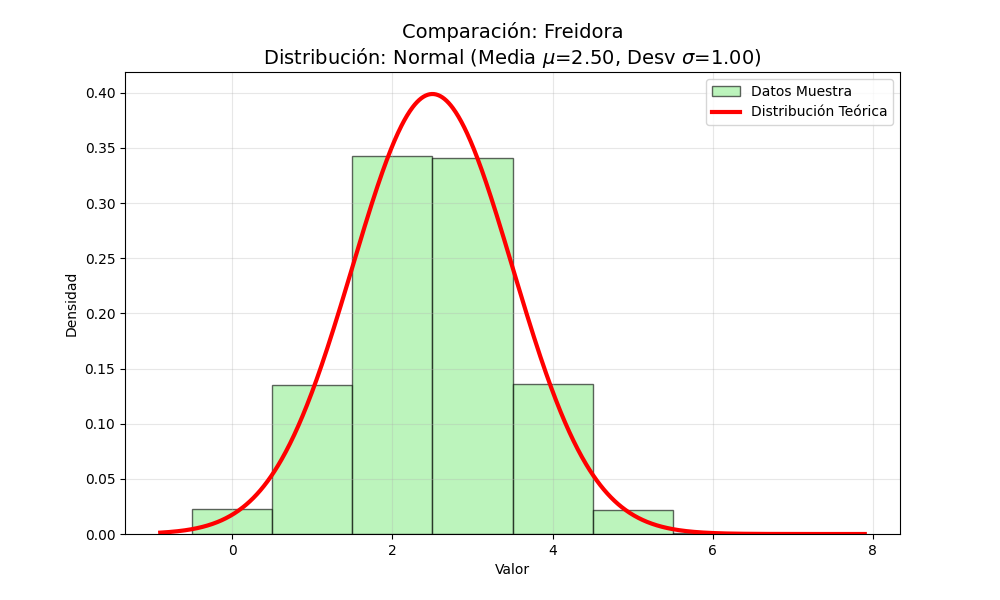
\includegraphics[width=\linewidth]{Imágenes/compara/freidoraCompara.png}
        \caption{Comparación de la muestra}
        \label{fig:compara_freidora}
    \end{subfigure}
    \caption{Histogramas para el servicio de freidora.}
    \label{fig:hist_freidora}
\end{figure}

\begin{figure}[H]
    \centering
    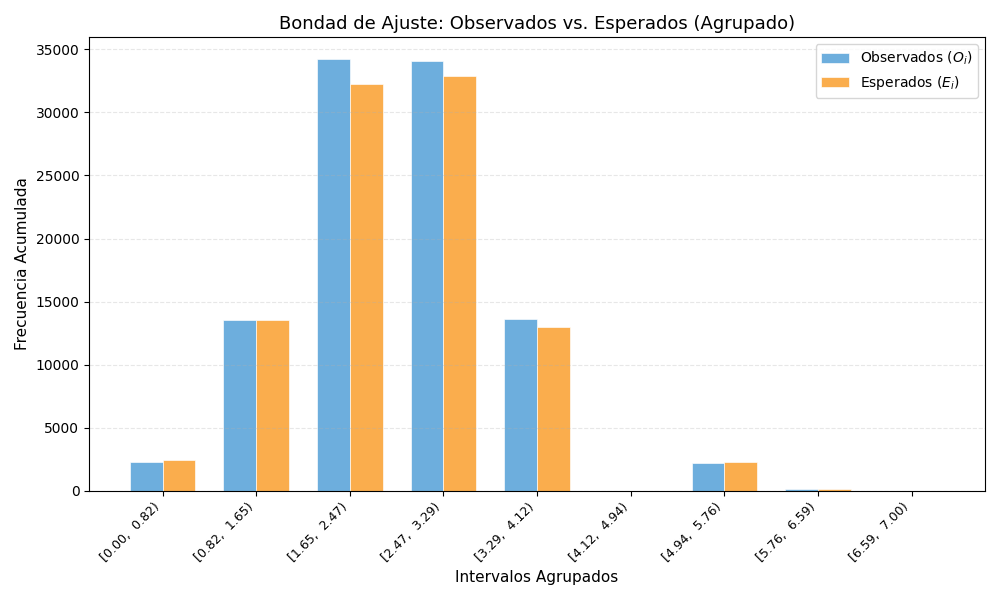
\includegraphics[width=0.5\textwidth]{Imágenes/obsEspe/freidoraObsEspe.png}
    \caption{Observados vs Esperados para freidora.}
    \label{fig:obsEspe_freidora}
\end{figure}

\begin{center}
    \textbf{Datos de la muestra (Freidora):}
    \vspace{0.2cm}
    \\Media (\(\mu\)): 2.5029 \quad | \quad Desviación (\(\sigma\)): 1.0351
\end{center}

\newpage
\subsubsection*{1.7.2.\hspace{0.5em} Planteamiento de hipótesis}
En base al análisis de los datos, se proponen las siguientes hipótesis:
\begin{center}
    \textbf{\(H_0\):} Esta es una distribución \textbf{Normal Discreta} con
    \(\mu = 2.5029\) y \(\sigma = 1.0351\).\\[0.5em]
    \textbf{\(H_1\):} La anterior \textbf{NO} es una buena descripción
    de la distribución.
\end{center}

\vspace{0.3cm}
\noindent \textbf{Criterios de decisión:}
\begin{itemize}
    \item Para la prueba \(\chi^2\): un nivel de confianza de \(95\%\) (\(\alpha = 0.05\)).
    \item Para la prueba \textit{Kolmogorov-Smirnov}: un nivel de confianza de \(95\%\) (\(\alpha = 0.05\)).
    \item Si \(\chi^2 \leq \text{valorCritico}\) y \(d \leq \text{valorCritico}\), entonces se acepta \(H_0\).
    \item Si no se cumple lo anterior, se rechaza la hipótesis nula.
\end{itemize}

\subsubsection*{1.7.3.\hspace{0.5em} Pruebas de bondad de ajuste}
\vspace{0.2cm}
\begin{minipage}{0.40\textwidth}
    \textbf{Probabilidad de Masa (PMF):}
    \[
        P(X=x) \approx \int_{x-0.5}^{x+0.5} \phi(t; \mu, \sigma) dt
    \]
\end{minipage}
\begin{minipage}{0.45\textwidth}
    \textbf{Función de Distribución (CDF):}
    \[
        F(x) \approx \Phi\left(\frac{x+0.5-\mu}{\sigma}\right)
    \]
\end{minipage}

\noindent
\begin{minipage}[t]{0.48\textwidth}
    \textbf{1. Prueba de \(\chi^2\)}
    \vspace{0.3cm}
    \begin{itemize}[itemsep=0.4em]
        \item \textbf{Calculado \(\chi^2\):} 3.8954
        \item \textbf{Valor crítico:} 11.0705
    \end{itemize}

    \begin{center}
        \vspace{0.5cm}
        \(3.8954 \leq 11.0705\)
        \vspace{0.1cm}
        \\\textbf{Resultado: }
        \textcolor{green!60!black}{\textbf{Aprobado}}
    \end{center}

    \vspace{0.8cm}

    \textbf{2. Prueba de Kolmogorov--Smirnov}
    \vspace{0.3cm}
    \begin{itemize}[itemsep=0.4em]
        \item \textbf{Calculado \(D\):} 0.001055
        \item \textbf{Valor crítico:} 0.004301
    \end{itemize}
    \begin{center}
        \vspace{0.5cm}
        \(0.0010 \leq 0.0043\)
        \vspace{0.1cm}
        \\\textbf{Resultado: }
        \textcolor{green!60!black}{\textbf{Aprobado}}
    \end{center}

\end{minipage}
\hfill
\begin{minipage}[t]{0.48\textwidth}
    \vspace{0pt}
    \centering
    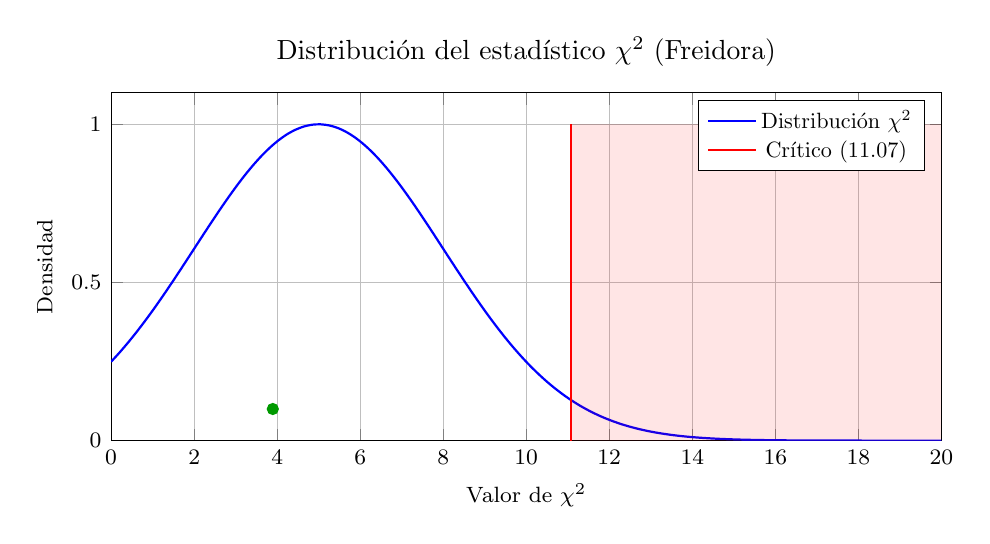
\begin{tikzpicture}
        \begin{axis}[
                width=\textwidth,
                height=6cm,
                title={Distribución del estadístico \(\chi^2\) (Freidora)},
                xlabel={Valor de \(\chi^2\)},
                ylabel={Densidad},
                xmin=0, xmax=20,
                ymin=0, ymax=1.1,
                grid=both,
                domain=0:20,
                samples=100,
                label style={font=\footnotesize},
                tick label style={font=\footnotesize},
                legend style={
                        nodes={scale=0.8, transform shape},
                        at={(0.98,0.98)},
                        anchor=north east
                    },]
            \addplot[blue, thick, smooth]
            {exp(-0.5*((x-5)/3)^2)};
            \addlegendentry{Distribución \(\chi^2\)}
            \addplot[red, thick]
            coordinates {(11.0705, 0) (11.0705, 1)};
            \addlegendentry{Crítico (11.07)}
            \addplot[fill=red, opacity=0.1]
            coordinates {(11.0705, 0) (20, 0) (20, 1) (11.0705, 1)};
            \addplot[
                mark=*,
                only marks,
                mark options={color=green!60!black, fill=green!60!black}
            ] coordinates {(3.8954, 0.1)};
        \end{axis}
    \end{tikzpicture}
\end{minipage}
\vspace{0.4cm}

\begin{center}
    Dado que ambas pruebas fueron aprobadas,
    \textbf{se acepta \(H_0\)}.
\end{center}